\documentclass[danish]{article}
\usepackage[utf8]{inputenc}
\usepackage[danish]{babel}
\usepackage[T1]{fontenc}	
\usepackage[a4paper, , margin=1in]{geometry}

\usepackage[version=3]{mhchem} % Package for chemical equation typesetting
\usepackage{siunitx} % Provides the \SI{}{} and \si{} command for typesetting SI units
\usepackage{graphicx} % Required for the inclusion of images
\usepackage{subcaption} % Add the possibility for subfigures/subcaptions.
\usepackage{natbib} % Required to change bibliography style to APA
\usepackage{amsmath} % Required for some math elements
\usepackage{amssymb}
\usepackage{float}
\graphicspath{ {graphics/} }

\setlength\parindent{0pt} % Removes all indentation from paragraphs

\renewcommand{\labelenumi}{\alph{enumi}.} % Make numbering in the enumerate environment by letter rather than number (e.g. section 6)
\begin{document}

\title{\textbf{Introduktion til Digital Signalanalyse }   Eksamensforberedelse}
\author{Jonas Lind}
\date{15-08-2017}
\maketitle
\section{Analyse af digitale signaler med Diskret Fourier Transformation og Spektrogram}

\section{Spektral forbredning, zero-padding og window functions i relation til DFT}

\section{FIR/IIR filter analyse og design vha. placering af poler/nuller i pol-nulpunkts-diagrammet}

\section{Window method til FIR filter design}

\section{Interpolation og decimation}

\section{Differentiation og integration}

\section{Stokastiske signaler, herunder middelværdi, varians, sandsynligheds-tæthedsfunktion og histogram}

\section{Beregning af Signal-Noise Ratio i tids- og frekvens-domænet}

\section{Midlingsfiltre}

\newpage
\section{Auto- og kryds-korrelation}
\subsection{Foldning}
Foldning er en matematisk måde at kombinere to signaler til at danne et tredje signal.
\subsubsection{Delta Funktion og Impuls Respons}
\begin{itemize}
	\item Delta-funktionen $\delta[n]$ er en normaliseret impuls.
	\item Alle dens samples har en værdi på 0, bortset fra samplenummer 0, som har en værdi på 1.
	\item Impuls responset $h[n]$ for et lineært system er outputtet fra systemet, når inputtet er en delta-funktion.
\end{itemize}

\begin{figure} [H]
	\centering
	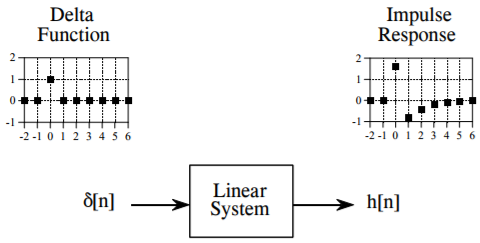
\includegraphics[width=0.6\linewidth]{graphics/deltafunction_impulseresponse}
	\caption{Definition af delta funktionen og impuls responset.}
	\label{fig:deltafunction_impulseresponse}
\end{figure}

\begin{itemize}
	\item Inputsignalet foldet med systemets impuls respons er svarende til outputsignalet.
	\item Hvis x[n] er et signal med N antal samples fra 0
	til N-1, og h[n] er et signal med M antal samples fra 0 til M-1, bliver foldningen af de to signaler:  $y(n) = x(n) \circledast y(n)$, et signal med $N+M-1$ antal samples fra 0 til $N+M-2$.
\end{itemize}

\begin{equation}
y(n) = \sum_{k=0}^{M-1} h(k) \cdot x(n-k) = h(n) \circledast x(n)
\end{equation}

\begin{itemize}
	\item Inputsignalet x(k) flippes rundt så dette placerer
	sample 0 til højre og efterfølgende opadgående samples til venstre.
	\begin{itemize}
		\item x(k) bliver herved til x(-k).
	\end{itemize}
	\item Alle produkter af h(k) og x(0-k) for alle k-værdier summeres og herved fås y(0).
	\item x(-k) shiftes en sample til højre.
	\item  Alle produkter af h(k) og x(1-k) for alle k-værdier summeres og herved fås y(1).
	\item Der shiftes og summeres indtil der ikke er overlap mellem h(k) og x(n-k).
\end{itemize}

\begin{figure}[H]
	\centering
	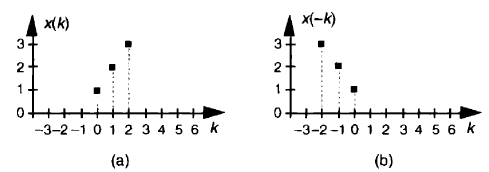
\includegraphics[width=0.6\linewidth]{graphics/convolution}
	\caption{(a) sekvensen $x(k)$; (b) spejling af sekvensen $x(k)$ omkring $k = 0$.}
	\label{fig:convolution}
\end{figure}

\textbf{Foldnings‐teorem I} betyder at foldning af to signaler i tidsdomænet er det samme som multiplikation af to signaler i frekvensdomænet.

\begin{equation}
h(n) \circledast x(n) \Leftrightarrow H(e^{j\omega}) \cdot X(e^{j\omega})
\end{equation}

\textbf{Foldnings-teorem II} betyder at foldning af to signaler i frekvensdomænet er det samme som multiplikation af to signaler i tidsdomænet. 

\begin{equation}
h(n) \cdot x(n) \Leftrightarrow H(e^{j\omega}) \circledast X(e^{j\omega})
\end{equation}

\subsection{Krydskorrelation}
Korrelation mellem 2 signaler.
Kan bruges til at finde periodicitet i et signal, signaldetektion eller system identifikation

\begin{itemize}
	\item Amplituden af hver sample i krydskorrelationssignalet er mål for hvor meget det signal der er optaget lignet det oprindelige target signal.
	\item r(n) er derfor et mål for, hvor meget et signal ligner et andet signal - tidsforskudt med n.
\end{itemize}
\begin{equation}
r(n) = \sum_{k=-\infty}^{\infty} h(k) \cdot x(n+k) = h(n) \circledast x(-n)
\end{equation}

\begin{figure}[H]
	\centering
	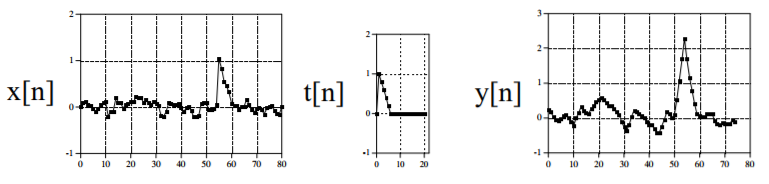
\includegraphics[width=0.8\linewidth]{graphics/crosscorrelation}
	\caption{y(n) er krydskorrelationen mellem x(n) og t(n).}
	\label{fig:crosscorrelation}
\end{figure}

\subsection{Autokorrelation}
Korrelation af signal med sig selv tidsforskudt.

\begin{equation}
r(n) = \sum_{k=-\infty}^{\infty} x(k) \cdot x(n+k) = x(n) \circledast x(-n)
\end{equation}

\newpage
\section{CASE projekt 1 – FSK transmission}

\section{CASE projekt 2 – Audio filter}

\section{CASE projekt 3 – Vejecelle}

\newpage
\section{CASE projekt 4 - Sonar}
\subsection{Opgavebeskrivelse}
\begin{itemize}
	\item Afstandsbestemmelse ved et udsende et akustisk signal.
	\item Systemet vil afspille og optage ekko-signalet på Blackfin kittet.
	\item Afstanden findes ved hjælp af krydskorrelation. 
\end{itemize}
	
\subsection{Signal generation}
\begin{itemize}
	\item Krav til signalet er at samplefrekvensen er \SI{48}{\kilo\hertz}, da det er denne som Blackfin kittet arbejder med. Vi vælger \SI{50}{\milli\second} og derfor får vi en arraystørrelse på 2400 samples.
	\item Et unikt signal ønskes, hvorfor et sweep eller hvid støj er bedre end et sinus signal. 
	\begin{itemize}
		\item Et sinus signal er kontinuert og da den gentager sig selv er det et problem da vi med korrelation leder efter gentagelser.
	\end{itemize} 
	\item Længden af signalet skal sørge for at være langt nok til at optage både når signalet sendes afsted og indtil det er kommet tilbage. 
	\item Præcisionen af målingen er $\frac{\SI{340}{\meter\per\second}}{\SI{48}{\kilo\hertz}} \approx \SI{7}{\milli\meter}$ per sample.
	\item Systemet skal kunne måle afstande op til \SI{10}{\meter}. Dette giver en forventning om at ekkoet skal rejse \SI{20}{\meter}, hvilket tager $\frac{\SI{20}{\meter}}{\SI{340}{\meter\per\second}} \approx \SI{59}{\milli\second}$.
	\item Antal samples der er brug for til at optage afspilningen er $F_s \cdot T + 2400 \cdot 2 \approx 7600$.
	\item Optagetiden er herved $\frac{7600}{F_s} \approx \SI{160}{\milli\second}$.
	\item Array størrelsen bliver hermed $2^{13} = 8192$.
\end{itemize}

\subsection{Signal analyse}

\end{document}